\chapter{Flash Analysis}
\label{chp:Flash_Analysis}

%checklist:
% - introduction (goal)
% - Test setup
% - Proceedings in this chapter

The goal of this chapter is to find a method, capable of obtaining consistent measures of the environment from measured flashes. Additional goals are to achieve this with the shortest flash and with the least complex method as possible. 

In this chapter, the platform is set-up as seen in figure \ref{fig:Flashcapturing}. D in the figure represents the distance between the device and the reflecting surface. all measurements have been placed in a darkroom, a room where no lights from outside can enter, so the test result won't get influenced by other illumination sources.
 
The set-up will first be used to get a reasonable understanding of what flashes look like and how settings of the flash generator influence the received flash. Then, several methods of obtaining these information flashes will be presented and compared. This chapter will conclude with a final settings used in the flash generator and an algorithm to obtain a consistent measure of the environment from the received flash.
\begin{figure}
	\centering     %%% not \center
	\label{fig:Flashcapturing}
	\subfigure[Test setup in illuminated environment]{\label{fig:a}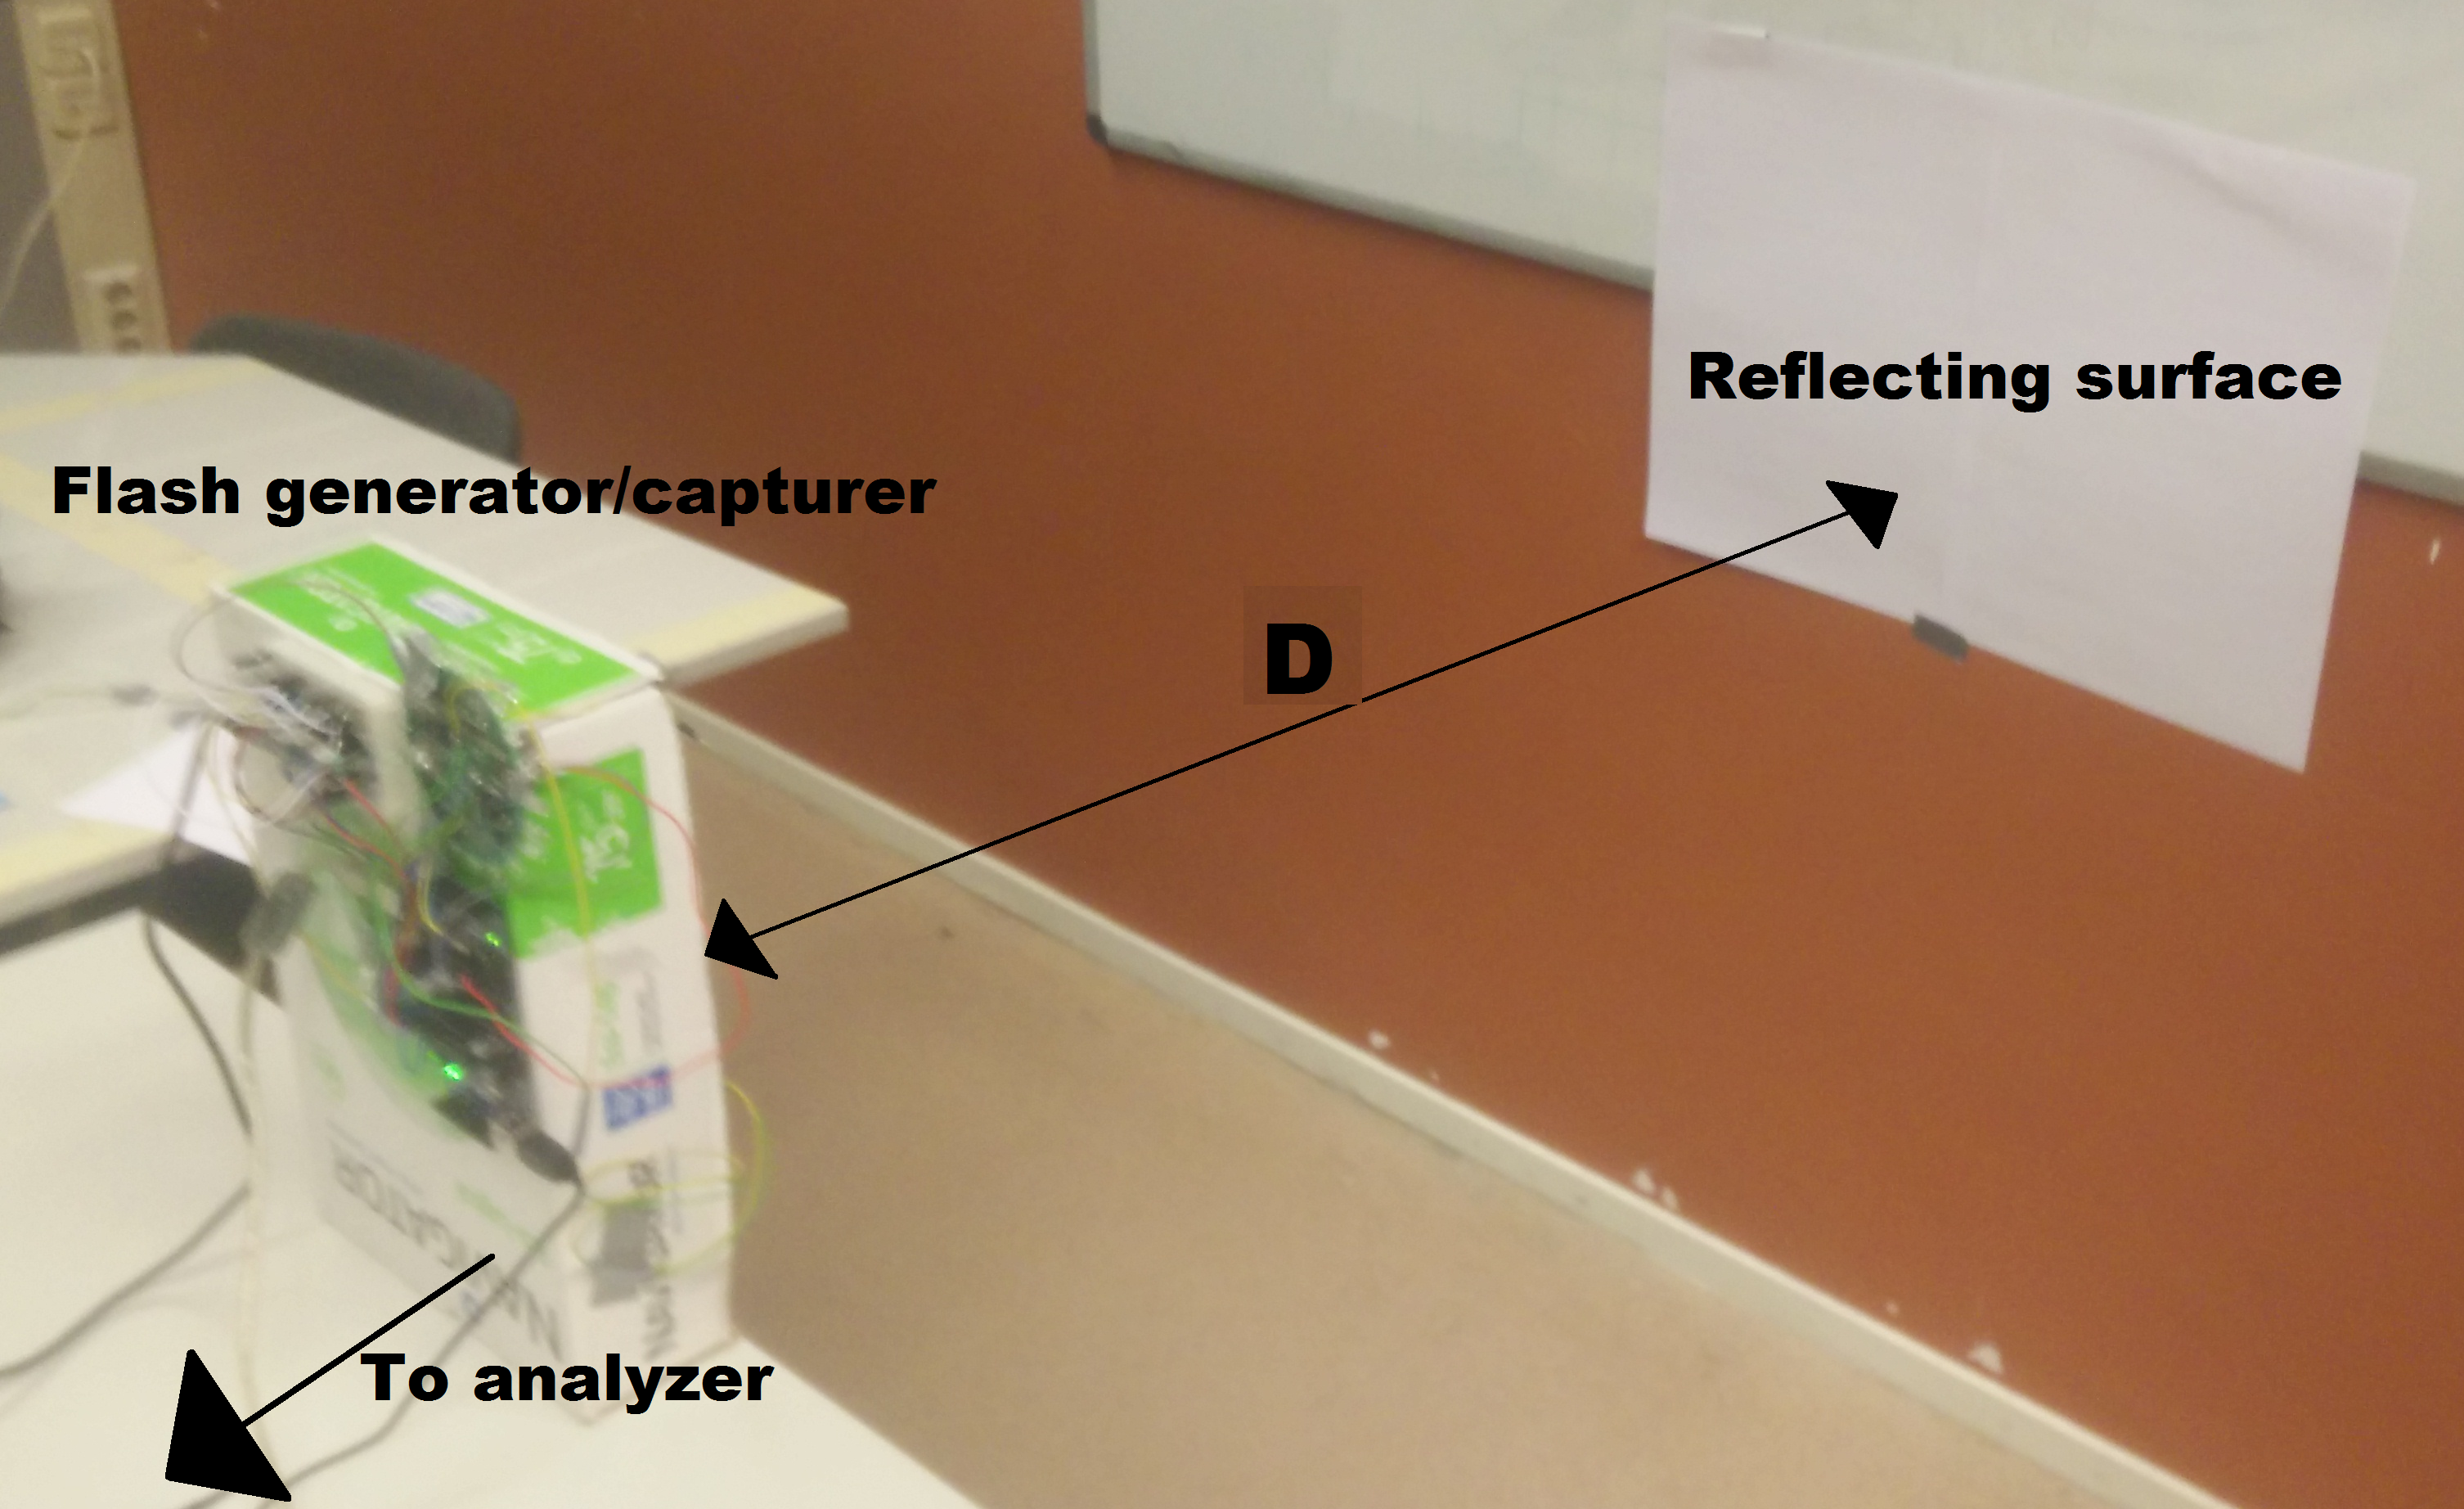
\includegraphics[width=60mm]{pics/Flashcapture_light.png}}
	\subfigure[Test set-up in dark environment]{\label{fig:b}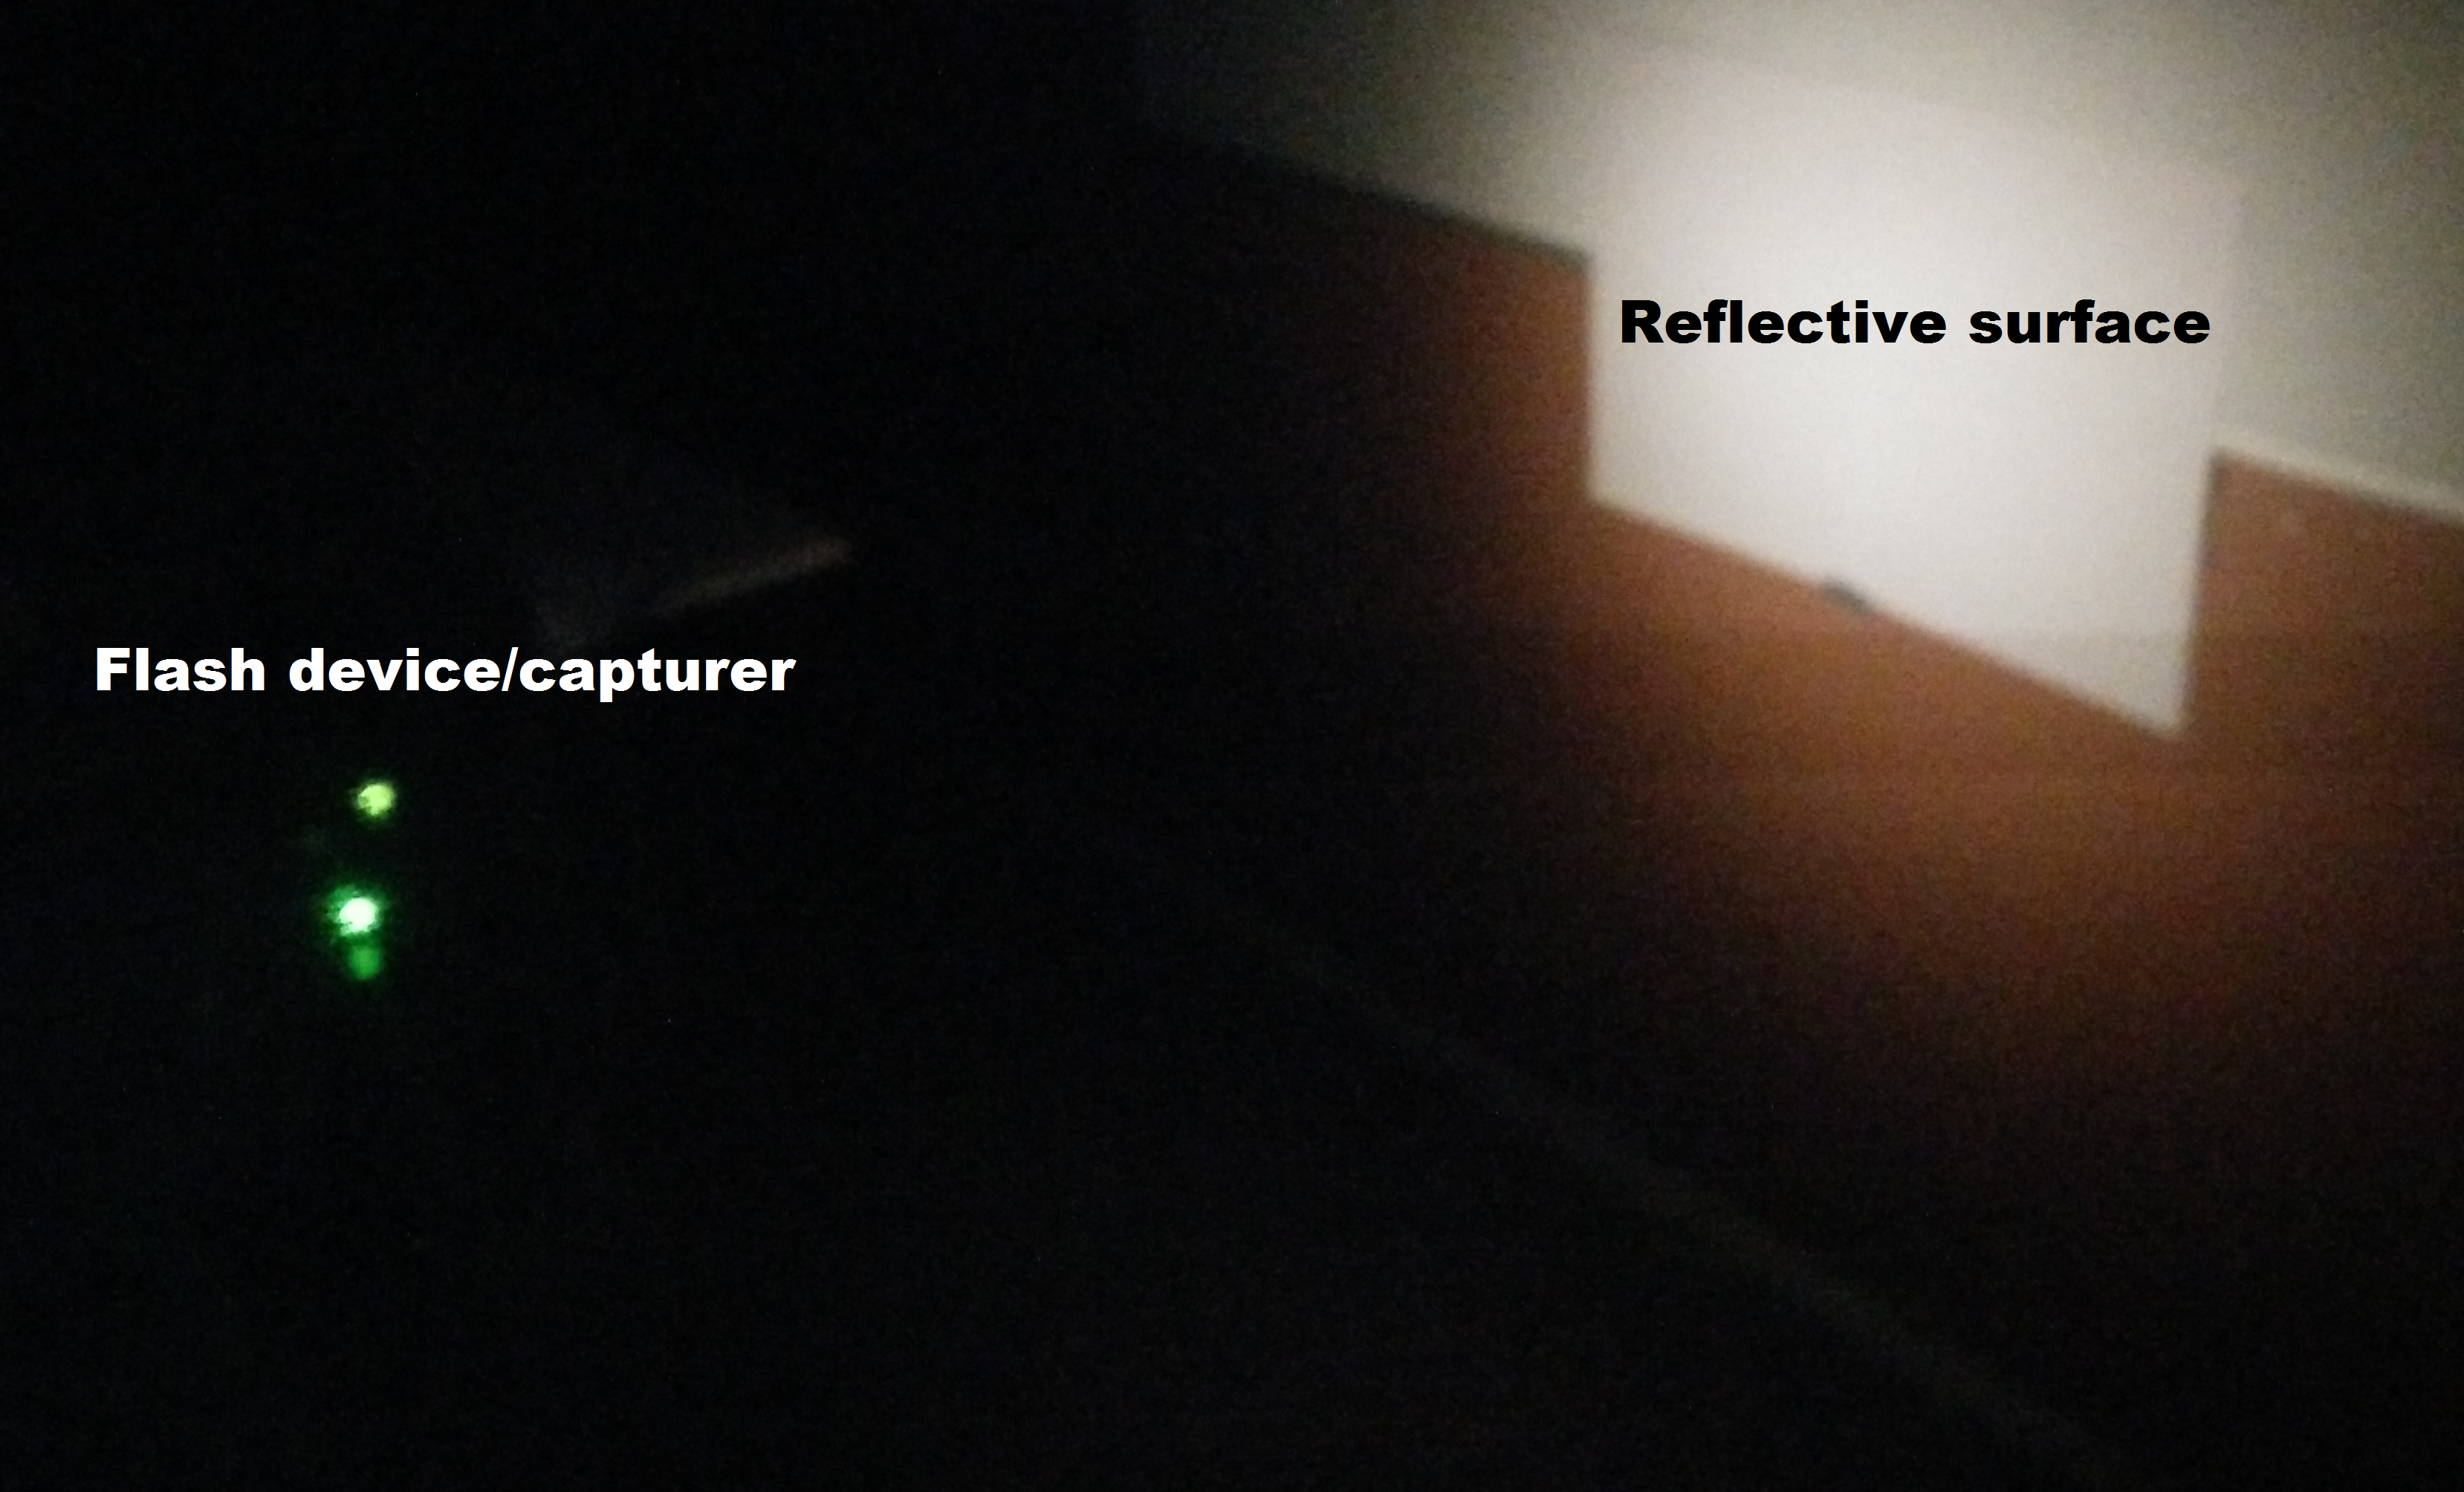
\includegraphics[width=60mm]{pics/Flashcapture_dark.png}}
	\caption{Test set-up used to capture flashes in the darkroom.}
\end{figure}

\section{Flash properties}
\label{sec:Flash_generator}
The test set-up has several parameters which can affect the perceived flash: $T_{on}$ (on time of the LED), $I$ (brightness of the LED), $PD$ (sensitivity of the photo diode) and $D$ (distance between device and reflecting surface). This section shows how each of these parameters influences the received signal. Note that the period, $T$, is not present in the list as should not influence an individual flash, but only the total amount of flashes.

Figure \ref{fig:InfOfTon} shows several responses for different $T_{on}$. In the figure it can be seen that all signals closely match each other, until the light is turned off. This is a useful property as this means it's possible to reduce the $T_{on}$ with no influence on the signal, if the last part is not used.

Figure \ref{fig:InfOfI} shows the influence of using the different amplification circuits of the flash generator. It can be seen that the LED powered with the lower resistance (and thus a higher LED current) is perceived as brighter to the system than the lights powered with a bigger resistor. It's also observed that the LED powered with higher currents show up earlier to the system. This is because LEDs driven with higher currents turn on faster \cite{LED_on}. This means that if a lower LED current is used a bigger $T_on$ is required to obtain useful information.

Figure \ref{fig:InfOfD} shows a set of measured flashes at a variance distance from the wall. It clearly shows that if the distance increases, the observed light also decreases. This is logical, as when light longer distances, the relative intensity of the light decreases. 
\begin{figure}
	\centering     %%% not \center
	\label{fig:InfOf}
	\subfigure[Sideview]{\label{fig:InfOfTon}\includegraphics[width=60mm]{pics/InfluenceOfTon.png}}
	\subfigure[Topview]{\label{fig:InfOfI}\includegraphics[width=60mm]{pics/InfluenceOfI.png}}
	\\
	\subfigure[Topview]{\label{fig:InfOfD}\includegraphics[width=60mm]{pics/InfluenceOfD.png}}
	\caption{Several perceived flashes generated with different settigns of $T_{on}$, $I_{LED}$ and $D$.}
\end{figure}

% properites checklist:
% - What happens if distance increases
%   + fig with multiple distances
% - What happens if t-on time increases
%   + fig with increasing t-on
% - What happens if intensity increases
%   + fig multiple 3 intensities
% sumarize in table 
% conclude:
% - 



\section{Flash features}
This section explores what kind of features can be extracted from a flash signal. It will then compare the methods based on required $T_{on}$, precision, the "Signal to Noise Ratio" (SNR) and computational complexity.

\subsection{Feature considerations}
The maximum of a flash response could contain useful information. Even though the light at the first maximum has not fully turned on yet, it still is some measure of the perceived light. This can be especially useful if the maximum of the flash always occurs at the exact same moment in time relative to the light turning on. If that is the case, then the maximum value of the first peak could provide us with enough information of the environment. If the maximum value of the first peak holds enough information, then a very small $T_{on}$ can be used to obtain this value, as decreasing $T_{on}$ does not significantly influence the height and form of the first peak.

Another possibility is the to remove the oscillation of the signal with a low pass filter and then take the maximum value of the filtered signal. This method less reliant on precise timing of the pulse. It also uses more samples of the signal and should therefore be able to obtain a value which better represents the reflections of the current environment than the maximum method.

Another method considered is to use the surface underneath the signal. This method has the advantage of being both simple and flexible. It does not matter if $T_{on}$ is chosen big or small, this method always uses all information available to obtain a measure of the reflections.

The final possibility considered is the filtered sum method. It first uses a filter to smooth the signal to then calculated the surface underneath it. This method could lead to more precise measures of the reflections as it uses more samples of the signal, and removes the ripple from the signal.

\subsection{Feature comparison}


\section{Selection of system parameters}
% - Compare explored methods on and SNR (std vs max std of mean), Energy used (required t-on),
% - Choose method
% - Choose sample reuqency

The final parameter to decide is the period of the signal $T$. This value has no influence on the noise measured on the signal except for the frequency. It has however a clear influence on how much light is used by the system, as decreasing $T$ directly increases the amount of flashes. We can't choose a too low value for $T$ as then users will observe flickering of the light. Another reason $T$ can't be chosen too low is that certain kind of noise still needs to be filtered out of the system. It is almost guaranteed that some 50Hz component will be seen in the signal, as long as its connected to the net. 

For these reasons, $T$ was chosen to be 800$\mu s$. This value results in a flash frequency of 125Hz. This value is more that the Nyquist frequency of the 50Hz. Even though literature recommends at least 200Hz to prevent the visibility of flickering, none was observed by 10 different test subjects with this setting of $T$. Another benefit is that the found method does not require a lot of computational power.

\section{Conclusion}
The Flash analyser will run at a frequency of 125Hz and a $T_on$ of $140\mu s$. The intensity of the light will be selected when the system is tested on full scale so that the signal does not saturate. These settings provide a reasonable level of precision. The next step for the project is creating an algorithm for the analyser, capable of analysing a set of consecutive flashes as seen in figure X.